\documentclass[11pt]{article}
\usepackage[sort]{natbib}
\usepackage{bm,amsmath,bbm,amsfonts,nicefrac,latexsym,amsmath,amsfonts,amsbsy,amscd,amsxtra,amsgen,amsopn,bbm,amsthm,amssymb,graphicx}
\usepackage{fancyhdr}
\usepackage[margin=1.0in]{geometry}
\bibliographystyle{plainnat}

\title{Improvement of forest carbon balance model DALEC2 for flux site Alice Holt using four-dimensional variational data assimilation.}
\author{Ewan Pinnington}

\newtheorem{theorem}{Theorem}[section]
\newtheorem*{defn}{Definition}


\begin{document}

\maketitle

\section{Introdution}

Four-dimensional variational data assimilation (4D-Var) has been used extensively in numerical weather prediction to improve forecasts REF. Currently efforts to use variational assimilation with carbon balance models have been limited REF, with sequential and Markov Chain Monte Carlo methods being more prevelant REF. In this report we will paramterize a model of forest carbon balance (DALEC2) using a 4D-Var scheme in order to produce better forecasts of forest carbon balance. We will use data from the research site at Alice Holt forest run by Forest Research.  

\section{Methods}

\subsection{4D-Var}

In 4D-Var we aim to maximise the probability of our initial state $\textbf{x}_0$ given a set of observations $\textbf{y}$, $P(\textbf{x}_0|\textbf{y})$, over some time window, $N$. $P(\textbf{x}_0|\textbf{y})$ is maximised by minimising a cost function $J(\textbf{x})$ derived from Baye's Theorem \citep{lewis2006dynamic}. The cost function is given as,

\begin{equation}
J(\textbf{x}_0) = \frac{1}{2}(\textbf{x}_0-\textbf{x}_b)^{T}\textbf{B}^{-1}(\textbf{x}_0-\textbf{x}_b)+\frac{1}{2}\sum_{i=0}^{N}(\textbf{y}_i-h_i(\textbf{x}_i))^{T}\textbf{R}_{i}^{-1}(\textbf{y}_i-h_i(\textbf{x}_i)),
\end{equation}•
where $\textbf{x}_b$ is our background and acts as our initial guess to our state $\textbf{x}_0$, $\textbf{B}$ is the background error covariance matrix and quantifies our knowledge of the error in our background, $h_i$ is our observation operator at time $t_i$ and maps our state vector evolved by our nonlinear model ($m_{0\rightarrow i}(\mathbf{x}_{0})=\textbf{x}_i$) to the observations at this time $\textbf{y}_i$ and $\textbf{R}_i$ is the observation error covariance matrix and represents our knowledge of the uncertainty in the observations. The state that minimises the cost function is called the analysis and is denoted as $\textbf{x}_a$, this state is found using a minimisation routine that takes the cost function, our initial guess ($\textbf{x}_b$) and also the gradient of the cost function defined as,

\begin{equation}
\nabla J(\textbf{x}_0) = \textbf{B}^{-1}(\textbf{x}_0-\textbf{x}_b)-\sum_{i=0}^{N}\textbf{M}_{i,0}^{T}\textbf{H}_i^{T}\textbf{R}_{i}^{-1}(\textbf{y}_i-h_i(\textbf{x}_i)),
\end{equation}•
where $\textbf{H}_i = \frac{\delta h_i(\textbf{x}_i)}{\delta\textbf{x}_i}$ is our linearized observation operator and $\mathbf{M}_{i,0}=\mathbf{M}_{i-1}\mathbf{M}_{i-2}\cdots\mathbf{M}_0$ is our tangent linear model with $\mathbf{M}_i=\frac{\delta m_{i}(\textbf{x}_{i})}{\delta \textbf{x}_{i}}$. 

\subsection{The DALEC2 model}

The DALEC2 model is a simple process-based model describing the carbon balance of a forest ecosystem \citep{Bloom2014} and is the new version of the original DALEC \citep{williams2005improved}. The model is constructed of six carbon pools (labile ($C_{lab}$), foliage ($C_f$), fine roots ($C_r$), woody stems and coarse roots ($C_w$), fresh leaf and fine root litter ($C_l$) and soil organic matter and coarse woody debris ($C_s$)) linked via fluxes. The aggregated canopy model (ACM) \citep{williams1997predicting} is used to calculate daily gross primary production ($GPP$) of the forest, taking meteorological driving data and the site's leaf area index (a function of $C_f$) as arguments.   

\begin{figure}[ht]
    \centering
    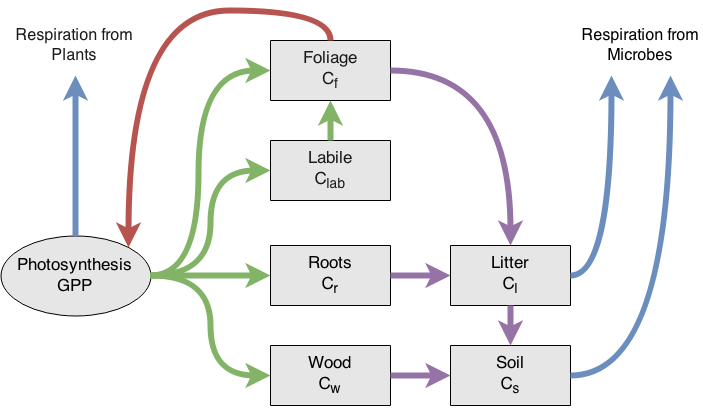
\includegraphics[width=0.5\textwidth]{Dalecdiagram.png}
    \caption{Representation of the fluxes in the DALEC2 carbon balance model. Green arrows represent C allocation, purple arrows represent litterfall and decomposition fluxes, blue arrows represent respiration fluxes and the red arrow represents the feedback of foliar carbon to the $GPP$ function.}
    \label{fig:DALEC_mod}
\end{figure}

The model equations for the carbon pools at day $t+1$ are as follows:

\begin{align}
GPP^{t} &= ACM(C_f^{t}, c_{lma}, c_{eff}, \Psi)
\\C_{lab}^{t+1}&=(1-\Phi _{on})C_{lab}^{t}+(1-f_{auto})(1-f_{fol})f_{lab}GPP^{t}, \label{daleclab}
\\C_f^{t+1}&=(1-\Phi_{off})C_f^{t}+\Phi_{on}C_{lab}^{t}+(1-f_{auto})f_{fol}GPP^{t}, \label{dalec1}
\\C_r^{t+1}&=(1-\theta_{roo})C_r^{t}+(1-f_{auto})(1-f_{fol})(1-f_{lab})f_{roo}GPP^{t}, 
\\C_w^{t+1}&=(1-\theta_{woo})C_w^{t}+(1-f_{auto})(1-f_{fol})(1-f_{lab})(1-f_{roo})GPP^{t}, 
\\C_l^{t+1}&=(1-(\theta_{lit}+\theta_{min})e^{\Theta T^{t}})C_l^{t}+\theta_{roo}C_r^{t}+\Phi_{off}C_f^{t}, 
\\C_s^{t+1}&=(1-\theta_{som}e^{\Theta T^{t}})C_s^{t}+\theta_{woo}C_w^{t}+\theta_{min}e^{\Theta T^{t}}C_l^{t}, \label{dalec5}
\end{align}

where $T^{t}$ is the daily mean temperature, $p_1,\ldots,p_{10}$ are rate parameters and $\phi$ represents the meteorological driving data used in the $GPP$ function. The full details of this version of DALEC can be found in \cite{Bloom2014}. It is parameterized for data from a young pine stand in Ponderossa, Oregon. The model parameters and the equations used to calculate $GPP$ are included in the appendix. We now see how DALEC can be implemented in a four-dimensional variational data assimilation (4D-Var) framework.

Forecast skill score, $SS = 1 - \frac{MSE_{forecast}}{MSE_{ref}}$, %http://en.wikipedia.org/wiki/Forecast_skill



\bibliography{../PhD}{}
%\bibliographystyle{plain}

\end{document}